\chapter{Implementacija i korisničko sučelje}

\section{Korištene tehnologije i alati}

\paragraph{}
{Komunikacija u timu realizirana je korištenjem aplikacije WhatsApp1. Za izradu UML dijagrama korišten je alat Astah Professional2, a kao sustav za upravljanje izvornim kodom Git3. Udaljeni repozitorij projekta dostupan je na web platformi GitHub.
}
\paragraph{}{
Kao razvojno okruženje korišten je Microsoft Visual Studio5 - integrirano je razvojno sučelje (IDE) tvrtke Microsoft. Prvenstveno se koristi za razvoj računalnih programa za operacijski sustav Windows, kao i za web-stranice, web-aplikacije, web-usluge i mobilne aplikacije. Visual Studio za razvoj softvera koristi Microsoftove platforme kao što su windows API, Windows Forms, Windows Presentation Foundation, Windows Store i Microsoft Silverlight.
}
\paragraph{}{
Aplikacija je napisana koristeći radni okvir* jezik C\#6 za izradu backenda te React7 i jezik JavaScript za izradu frontenda. React, također poznat kao React.js je biblioteka u JavaScriptu za izgradnju korisničkih sučelja. Održana je od strane Facebooka. React se najčešće koristi kao osnova u razvoju web ili mobilnih aplikacija. Složene aplikacije u Reactu obično zahtijevaju korištenje dodatnih biblioteka za interakciju s API-jem. Radni okvir Baza podataka se nalazi na poslužitelju u oblaku Microsoft Azure.
}



\section{Ispitivanje programskog rješenja}

\section{Dijagram razmještaja}

\paragraph{}{
UML-dijagrami razmještaja (engl. deployment diagrams) prikazuju fizičku arhitekturu programskog sustava, prikazujući razmještaj programskih artefakata na sklopovskim čvorovima ili na virtualnim okruženjima.
}

\paragraph{}{
Naš se sustav bazira na ”klijent – posluzitelj” arhitekturi, te se komunikacija između računala korisnika i poslužitelja odvija pomoću HTTP veze. Pristup web aplikaciji odvija se preko web preglednika računala korisnika. Na poslužitelju se nalaze web poslužitelj i poslužitelj baze podataka.
}

\begin{figure}[!htb]
	\centering
	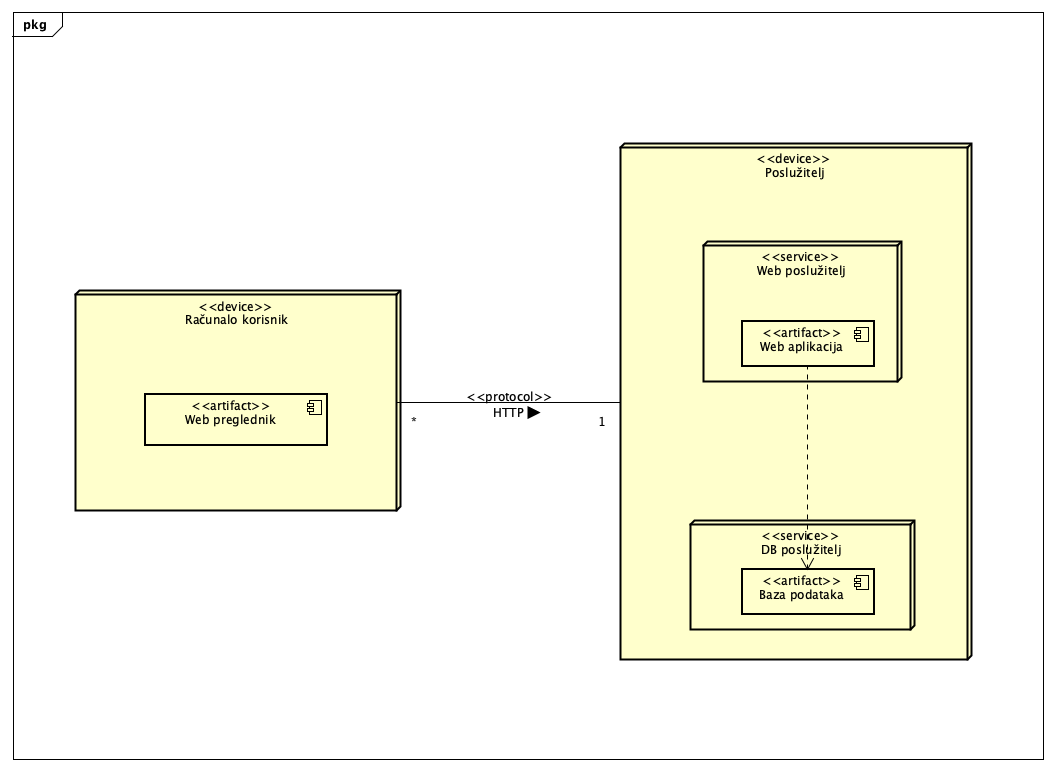
\includegraphics[width=1\linewidth]{dijagrami/DijagramRazmjestaja.png}
	\caption{Dijagram razmještaja}
	\label{fig:modelsdiagram}
\end{figure}

\section{upute za puštanje u pogon}


\eject